\documentclass[11pt,a4paper]{extarticle}
\usepackage[utf8]{inputenc}
\usepackage[spanish]{babel}
\usepackage{amsmath}
\usepackage{amsfonts}
\usepackage{amssymb}
\usepackage{graphicx}
\usepackage[left=1.2cm,right=1.2cm,top=2cm,bottom=2cm]{geometry}
\date{\small{\today}}
\usepackage{fancyhdr}
\usepackage{afterpage}
\usepackage{titlesec}
\usepackage{float}
\usepackage{gensymb}
\usepackage{xfrac}
\usepackage{tabularx}
\usepackage{multicol}
\usepackage[font=small]{caption}
\usepackage{scrextend}
\usepackage[toc,page]{appendix}

\renewcommand\appendixpagename{Apéndices}
\renewcommand\appendixname{Apéndice}

\titleformat{\section}{\Large\bfseries}{}{0em}{}[]
\titleformat{\subsection}{\large\bfseries}{}{0em}{}[]
\titleformat{\subsubsection}{\bfseries}{}{0em}{}[]
\titleformat{\chapter}{\large\bfseries}{}{0em}{}[]


\setlength\parindent{0pt}


\begin{document}
\title{Medición de Impedancias con Amplificador Lock In}
	\LARGE{\textsc{Laboratorio II}}\\
	\Large{Medición de Impedancias con Amplificador Lock In}\\
\begin{large}
\small\textsc{Horst, Raúl Tomás}\\
\small\textsc{Roqueta, Matías Daniel}\\
\small{Centro Atómico Bariloche y Instituto Balseiro, Comisión Nacional de Energía Atómica}\\
\end{large}
\setcounter{page}{1}

\lhead{Laboratorio II}%Materia
\rhead{Medición de Impedancias con Amplificador Lock In}%Título 
\chead{}

\lfoot{R. Horst, M. Roqueta}
\cfoot{Instituto Balseiro} 
\rfoot{\thepage} 
\renewcommand{\headrulewidth}{0.4pt} 
\renewcommand{\footrulewidth}{0.4pt} 
\pagestyle{fancy}

\hrule
\begin{multicols}{2}
\normalsize
\section{Resumen}

\section{Introducción}

Un amplificador lock in es un dispositvo electrónico capaz de extraer la fase y amplitud de una señal de banda angosta medida en un ambiente ruidoso.\\

El funcionamiento del lock in equiere información de la dependencia temporal de la señal de interés, que es aportada por una señal de referencia. Según la implementación, la señal de referencia puede ser inyectada al lock in de una fuente externa o generada internamente.\\ 

El lock in recupera la señal de interés multiplicando a esta por la referencia en fase y cuadratura, y aplicando un filtro pasa bajo al producto de señales. Este proceso es llamado \textit{demodulación coherente}.\\

\begin{figure}[H]
	\centering
	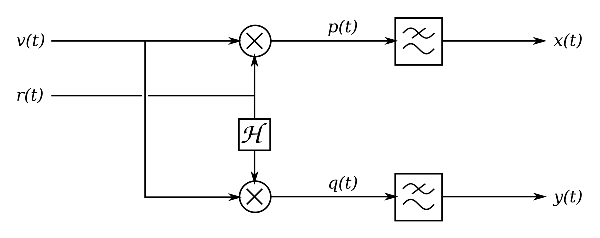
\includegraphics[width=\linewidth]{Images/lockin_gral.eps}
	\caption{Una señal de entrada $v(t)$ es inyectada al lock in. Posterior a la demodulación coherente, se extrae la señal de interés $z(t)=x(t)+jy(t)$}
	\label{fig:lockin}
\end{figure}

La figura \ref{fig:lockin} presenta un circuito lock in típico. El bloque transformada de Hilbert para una referencia senoidal corresponde a un desfasaje de 90°. La señal de salida se obtiene en forma de parte real e imaginaria, pero típicamente se expresa en forma amplitud y fase

\begin{equation*}
	z(t) = x(t) + j y(t) = R(t) e ^{j\Phi(t)}
\end{equation*}\\[-1em]

Donde la amplitud y fase se obtienen de las ecuaciones

\begin{equation*}
	R(t) = \sqrt{x^2(t)+y^2(t)} \qquad \qquad \Phi(t) = \arctan\frac{y(t)}{x(t)}
\end{equation*}\\


Para comprender el comportamiento esperando del demodulador coherente resulta útil visualizar las señales involucradas en el dominio de la frecuencia, análisis que se realiza en la figura \ref{fig:sigs_fourier}.

\begin{figure}[H]
	\centering
	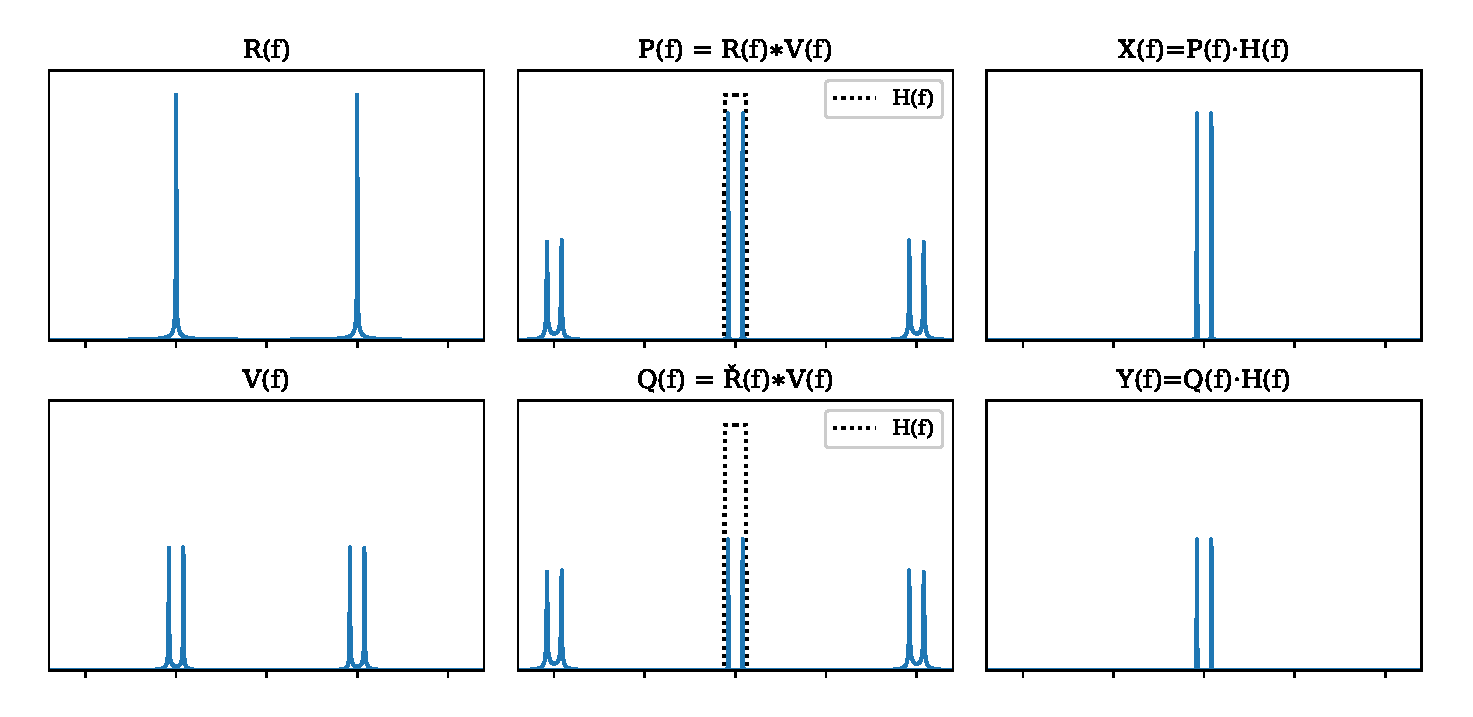
\includegraphics[width=\linewidth]{Images/sigs_fourier.eps}
	\caption{Realización en ausencia de ruido de las señales presentes en la figura \ref{fig:lockin} representadas en el dominio de la frecuencia, incluida la respuesta en frecuencia del filtro.}
	\label{fig:sigs_fourier}
\end{figure}

La salida $z(t)$ del demodulador coherente se puede interpretar como la entrada $v(t)$ transportada a banda base. Por este motivo la frecuencia de corte del filtro pasa bajos se debe elegir tal que acepte el ancho de banda de la señal a medir.

\section{Método Experimental}
\begin{figure}[H]
	\centering
	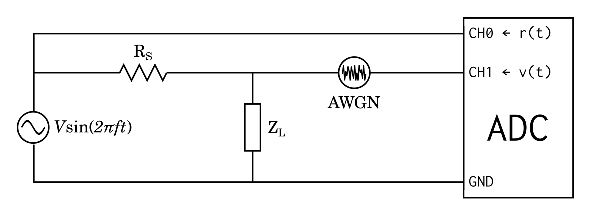
\includegraphics[width=\linewidth]{Images/circuito.eps}
	\caption{El circuito}
	\label{fig:circuito}
\end{figure}

En primer lugar se midió la frecuencia máxima de 
sampleo que permitía el dispositivo de medición.\\

Luego se ensambló el circuito de la figura \ref{fig:circuito}. sobre 
un protoboard. Con ésto se evaluó el funcionamiento del
lock-in en un circuito de carácter puramente resistivo 
en donde se pudo obtener el valor de la resistencia 
de carga RL.\\ 

Se utilizaron dos generadores de señal RIGOL DG4102 
para poder generar la señal de referencia y el ruido.
Para sumar éstas dos señales se tuvo que "flotar"[1] la 
tierra de uno de los generadores dado que éstos no poseen 
tierra propia, sino que utilizan la de la red eléctrica.\\

Para la realización del lock-in se implementó un 
script en python como se puede ver en el apéndice.
En el código se importó la librería del dispositivo 
de medición, el 
conversor analógico dígital USB-1408FS de la línea 
MEASUREMENT COMPUTING para poder 
calibrarlo y realizar las mediciones.\\

Se implementaron 
las etapas de la figura \ref{fig:lockin}, en donde 
se optó por utilizar filtros FIR dada su versatilidad 
y sencillez.

\section{Resultados}

Se determinó que la frecuencia máxima de muestreo es 
de aproximadamente 
500Hz, con una frecuencia máxima medible de 250Hz, 
según el teorema de uestreo de Nyquist[2].\\

Se midió el valor de RL en función 
de la relación señal a ruido en la entrada para tres 
filtros FIR de distintos orden.
Se puede apreciar que el filto óptimo es el de mayor 
orden, dado que se utilizan mayor cantidad de 
mediciones para generar las señales medidas.

\begin{figure}[H]
	\centering
	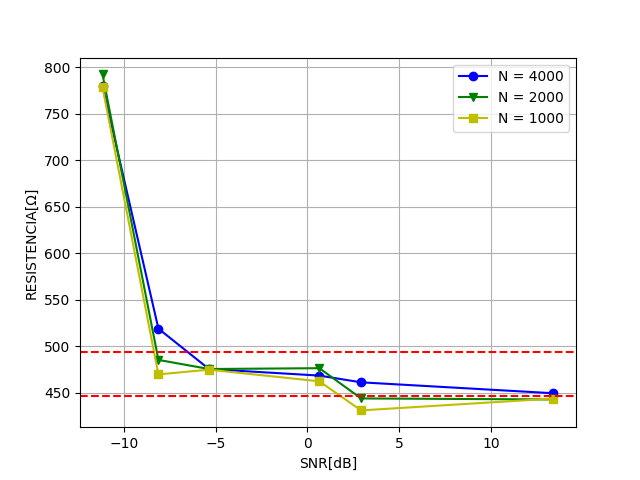
\includegraphics[width=\linewidth]{Images/RvsSNR(segunda).png}
	\caption{RvsSNR}
	\label{fig:RvsSNR}
\end{figure}

Para comprobar que el límite de funcionamiento 
del lock-in no está limitado por el orden del 
filtro elegido sino por la SNR a la entrada
se realizaron distintas mediciones 
sobre el valor RL(dada la simpleza del circuito) 
para un valor de SNR a la entrada de -22.5dB para 
distintos filtros como se explaya en la figura 
\ref{fig:RORDEN}. Se aprecia un valor mas acercado 
al tabulado cuando se aumenta el orden del filtro, sin 
embargo está lejos de entrar en la cota del error 
tabulado, y ésto afirma que el limitante en éste 
lock-in es el ruido a la entrada.\\

ESTARIA BUENO QUE EL ULTIMO PTO DE LA GRAFICA \ref{fig:RORDEN}
ESTE MAS ARRIBA PARA PODER HACER ESTA AFIRMACION 
VER SI CONVIENE PONER EN A TRABAJO FUTURO O MOVER EL PTO\\

\begin{figure}[H]
	\centering
	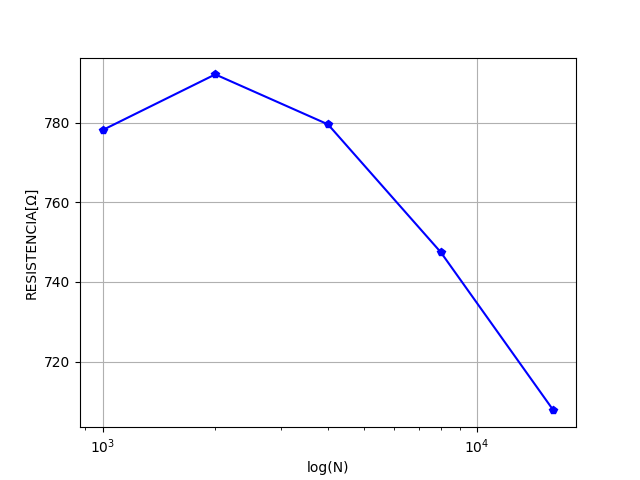
\includegraphics[width=\linewidth]{Images/RORDEN.png}
	\caption{RORDEN}
	\label{fig:RORDEN}
\end{figure}

Por último se armó el circutio de la figura 
\ref{fig:CvsSNR} .Con ésto 
se midió el valor de la capacidad CL para poder 
comprobar el funcionamiento del lock-in en 
impedancias complejas.

\begin{figure}[H]
	\centering
	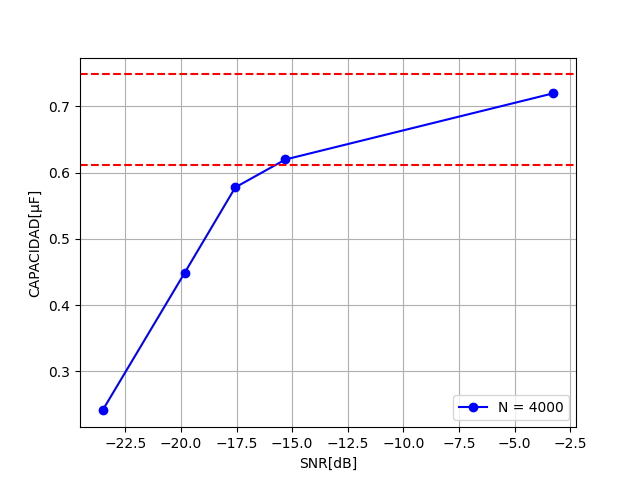
\includegraphics[width=\linewidth]{Images/CvsSNR(segunda).png}
	\caption{RvsSNR}
	\label{fig:CvsSNR}
\end{figure}


\section{Discusión}
-Orden del filtro\\
-Pq usamos FIR y no IIR\\
-Frecuencia de muestreo->usar otro dac\\
-Pq tuvimos que flotar\\

\section{Conclusiones}


\bibliography{Antenas}
\bibliographystyle{ieeetr}

\end{multicols}
\newpage
\begin{appendices}
\vspace{-1em}
\hrule
\vspace{1em}
\normalsize
\section{Apéndice 1 - si pinta meter un apéndice}
\end{appendices}

\end{document}
